\begin{center}
\begin{tabular}{c | c | c | c}
	Homeomorphism Class & Tree Indices & Homeomorphism Class & Tree Indices \\ \hline
	
\begin{tikzpicture}[scale=0.05, every node/.style={circle, inner sep=0pt, minimum size=2.5pt, fill=black}, level distance=4cm, level/.style={sibling distance=8cm/#1}]
		\node(root){}
			child {node{}};
	\end{tikzpicture} & (1,1) &
	
\begin{tikzpicture}[scale=0.05, every node/.style={circle, inner sep=0pt, minimum size=2.5pt, fill=black}, level distance=4cm, level/.style={sibling distance=8cm/#1}]
		\node(root){}
			child {node{}
				child {node{}}
				child {node{}}};
	\end{tikzpicture} & (1,2), (1,3), (1,4), (1,5) \\ \hline
		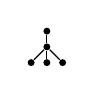
\begin{tikzpicture}[scale=0.05, every node/.style={circle, inner sep=0pt, minimum size=2.5pt, fill=black}, level distance=4cm, level/.style={sibling distance=8cm/#1}]
		\node(root){}
			child {node{}
				child {node{}}
				child {node{}}
				child {node{}}};
	\end{tikzpicture} & (1,6), (1,7), (1,8) &
	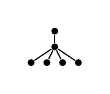
\begin{tikzpicture}[scale=0.05, every node/.style={circle, inner sep=0pt, minimum size=2.5pt, fill=black}, level distance=4cm, level/.style={sibling distance=8cm/#1}]
		\node(root){}
			child {node{}
				child {node{}}
				child {node{}}
				child {node{}}
				child {node{}}};
	\end{tikzpicture} & (2,1), (2,2) \\ \hline
 	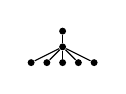
\begin{tikzpicture}[scale=0.05, every node/.style={circle, inner sep=0pt, minimum size=2.5pt, fill=black}, level distance=4cm, level/.style={sibling distance=8cm/#1}]
		\node(root){}
			child {node{}
				child {node{}}
				child {node{}}
				child {node{}}
				child {node{}}
				child {node{}}};
	\end{tikzpicture} & (2,3) &
	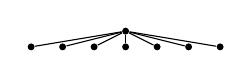
\begin{tikzpicture}[scale=0.05, every node/.style={circle, inner sep=0pt, minimum size=2.5pt, fill=black}, level distance=4cm, level/.style={sibling distance=8cm/#1}]
		\node(root){}
			child {node{}}
			child {node{}}
			child {node{}}
			child {node{}}
			child {node{}}
			child {node{}}
			child {node{}};
	\end{tikzpicture} & (2,4) \\ \hline
	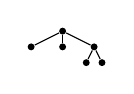
\begin{tikzpicture}[scale=0.05, every node/.style={circle, inner sep=0pt, minimum size=2.5pt, fill=black}, level distance=4cm, level/.style={sibling distance=8cm/#1}]
		\node(root){}
				child {node{}}
				child {node{}}
				child {node{}
					child {node{}}
					child {node{}}};
	\end{tikzpicture} & (2,5), (2,6), (2,7), (2,8), (3,1)&
	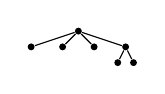
\begin{tikzpicture}[scale=0.05, every node/.style={circle, inner sep=0pt, minimum size=2.5pt, fill=black}, level distance=4cm, level/.style={sibling distance=8cm/#1}]
		\node(root){}
				child {node{}}
				child {node{}}
				child {node{}}
				child {node{}
					child {node{}}
					child {node{}}};
	\end{tikzpicture} & (3,2), (3,3), (3,4) \\ \hline
	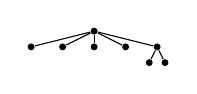
\begin{tikzpicture}[scale=0.05, every node/.style={circle, inner sep=0pt, minimum size=2.5pt, fill=black}, level distance=4cm, level/.style={sibling distance=8cm/#1}]
		\node(root){}
			child {node{}}
			child {node{}}
			child {node{}}
			child {node{}}
			child {node{}
				child {node{}}
				child {node{}}};
	\end{tikzpicture} & (3,5) &
	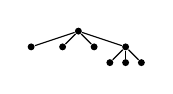
\begin{tikzpicture}[scale=0.05, every node/.style={circle, inner sep=0pt, minimum size=2.5pt, fill=black}, level distance=4cm, level/.style={sibling distance=8cm/#1}]
		\node(root){}
				child {node{}}
				child {node{}}
				child {node{}}
				child {node{}
					child {node{}}
					child {node{}}
					child {node{}}};
	\end{tikzpicture} & (3,6) \\ \hline
	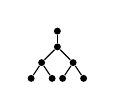
\begin{tikzpicture}[scale=0.05, every node/.style={circle, inner sep=0pt, minimum size=2.5pt, fill=black}, level distance=4cm, level/.style={sibling distance=16cm/#1}]
		\node(root){}
			child {node{}
				child {node{}
					child {node{}}
					child {node{}}}
				child {node{}
					child {node{}}
					child {node{}}}};
	\end{tikzpicture} & (3,7)

\end{tabular}
\end{center}

